\chapter{Elméleti megalapozás és szakirodalmi tanulmány}
\label{chap:elmelet}

Ebben a fejezetben azokat az elméleti és szakirodalmi alapokat foglalom össze, amelyek közvetlenül szükségesek a dolgozatban megvalósított hangszerfelismerő rendszer megértéséhez. Csak a projekt szempontjából lényeges témák kerülnek előtérbe: nem célom a teljes audio-jelfeldolgozás vagy mélytanulás részletes tárgyalása. Inkább azt mutatom meg, hogy a hang fizikai tulajdonságaiból hogyan jutok el a tanítható spektrogram-reprezentációkig, majd ezekből hogyan lesz osztályozó modell.

\section{Szakirodalmi és technológiai háttér}
\label{sec:szakirodalom}
\label{sec:technologiak}

Az automatikus hangszerfelismerés több, egymáshoz kapcsolódó területre épül: környezeti hangosztályozásra, zenei információ-visszakeresésre, izolált hangszerhangok elemzésére és neurális audio-reprezentációkra. A saját munkám szempontjából nem az volt a cél, hogy egy meglévő rendszert lemásoljak, hanem az, hogy ezekből a megközelítésekből kiválasszam azt az irányt, amely egy kis méretű, saját gyűjtésű, valós időben is használható rendszerhez illeszkedik.

A környezeti hangosztályozás egyik ismert kiindulópontja az ESC adathalmaz \cite{piczak2015esc}, amely rövid hangrészleteken vizsgálja a kategóriafelismerést. Ez a dolgozatban főleg a \textit{noise} osztály miatt fontos: a rendszernek nemcsak hangszercsaládokat kell felismernie, hanem azt is, amikor nincs értelmezhető hangszeres bemenet. A CNN-alapú környezeti hangosztályozásnál Salamon és Bello munkája különösen releváns, mert az adataugmentációt nem kiegészítő trükként, hanem a kis tanítóhalmazok általánosítását segítő eszközként vizsgálja \cite{salamon2017deep}. Közvetlenebb zenei előzmény az IRMAS adathalmaz \cite{bosch2012irmas}, amely már kifejezetten hangszerek felismerésére készült, zenei környezetben. Az én rendszerem ennél szűkebb feladatot vállal: rövid, egy másodperces mintákból hangszercsaládot becsül, mikrofonos használati helyzetre készülve.

Az izolált hangszerhangokat tartalmazó adathalmazok közül az NSynth \cite{engel2017nsynth}, a TinySOL \cite{cella2020tinysol}, a Medley-solos-DB \cite{lostanlen2018medley} és a GoodSounds \cite{romani2015good} adtak fontos támpontot. Ezek közös tanulsága, hogy a hangszín nem egyetlen egyszerűen mérhető érték, hanem az időbeli burkológörbe, a felharmonikus szerkezet, a megszólaltatási mód és a felvételi környezet együttese. Emiatt a saját rendszeremben nem sok különálló hangszert, hanem hét akusztikailag indokolható osztályt különítek el: gitár, zongora, vokál, vonós, nádfúvós, rézfúvós és zaj/csend.

A megvalósítás gyakorlati alapját Python környezetben a Librosa \cite{mcfee2015librosa}, a NumPy, a Matplotlib és a TensorFlow/Keras \cite{tensorflow2015-whitepaper} adta. A Librosa egységes módon támogatja a hullámformák betöltését, az STFT, MFCC és log-Mel reprezentációk előállítását, míg a TensorFlow/Keras a neurális modellek tanításához és kiértékeléséhez szolgált alapul. Az audio-jelfeldolgozási magyarázatoknál Valerio Velardo \textit{The Sound of AI} oktatási anyagát is felhasználtam \cite{velardo2020audio}. A YAMNet-alapú megközelítés az AudioSet nagyskálájú audioesemény-adatbázisához és az azon vizsgált CNN-alapú audioosztályozási irányhoz kapcsolódik \cite{gemmeke2017audioset,hershey2017cnn}; a dolgozatban nem a saját pipeline helyettesítője, hanem transzfer tanulási összehasonlítási pont.

\section{Digitális hang és hangreprezentáció}
\label{sec:elmeleti_alapok}

A hang fizikai értelemben időben változó nyomáshullám, amelyet a számítógép csak digitális mintasorozatként tud kezelni. A hangszerfelismerés szempontjából négy alapfogalom fontos: az \textbf{időtartam}, az \textbf{amplitúdó}, a \textbf{frekvencia} és a \textbf{hangszín}. Az időtartam azt írja le, meddig áll fenn a hang; az amplitúdó a jel kitérésének mértéke; a frekvencia a hangmagasság fizikai alapja; a hangszín pedig az a tulajdonság, amely alapján két azonos hangmagasságú és hangerejű hangot is meg tudunk különböztetni.

A hangszín szempontjából különösen fontos a felharmonikus szerkezet és az időbeli burkológörbe. A természetes hangszerek általában nem egyetlen frekvencián szólnak, hanem az alaphang mellett több felharmonikust is tartalmaznak. Emellett a hang felfutása, kitartása és lecsengése is erősen hangszerfüggő: egy zongorahang hirtelen indul és fokozatosan lecseng, míg egy vonós vagy fúvós hang hosszabban fenntartható.

A digitalizálás során az analóg hangból mintavételezéssel és kvantálással lesz diszkrét jelsorozat. A mintavételezési frekvencia azt adja meg, hogy másodpercenként hány ponton mérjük meg a jelet. A Nyquist-tétel alapján a rögzíthető legmagasabb frekvencia a mintavételezési frekvencia fele. A kvantálás az amplitúdóértékeket diszkrét szintekre kerekíti; ennek felbontását a bitmélység határozza meg.

\begin{table}[H]
\centering
\caption{A digitális hang legfontosabb alapparaméterei}
\label{tab:adc_params}
\begin{tabular}{p{4.0cm}p{3.0cm}p{6.3cm}}
\toprule
\textbf{Paraméter} & \textbf{Példaérték} & \textbf{Jelentés} \\
\midrule
Mintavételezési frekvencia & 16\,000 vagy 44\,100 Hz & Meghatározza az időbeli felbontást és a rögzíthető felső frekvenciatartományt. \\
Bitmélység & 16 bit & Meghatározza az amplitúdó felbontását és a dinamikatartományt. \\
Csatornaszám & mono / sztereó & A dolgozatban a feldolgozás egyszerűsítése miatt mono jeleket használok. \\
\bottomrule
\end{tabular}
\end{table}

A frekvenciaelemzéshez a folytonos mintasorozatot rövid, átfedő keretekre bontjuk. Ezt nevezzük keretezésnek. Mivel a keretek széleinél mesterséges megszakadások keletkezhetnek, az egyes keretekre ablakozó függvényt, például Hann-ablakot alkalmazunk. Ez csökkenti a spektrális szivárgást, vagyis azt a jelenséget, amikor a vágás miatt hamis frekvenciakomponensek jelennek meg.

\begin{figure}[H]
    \centering
    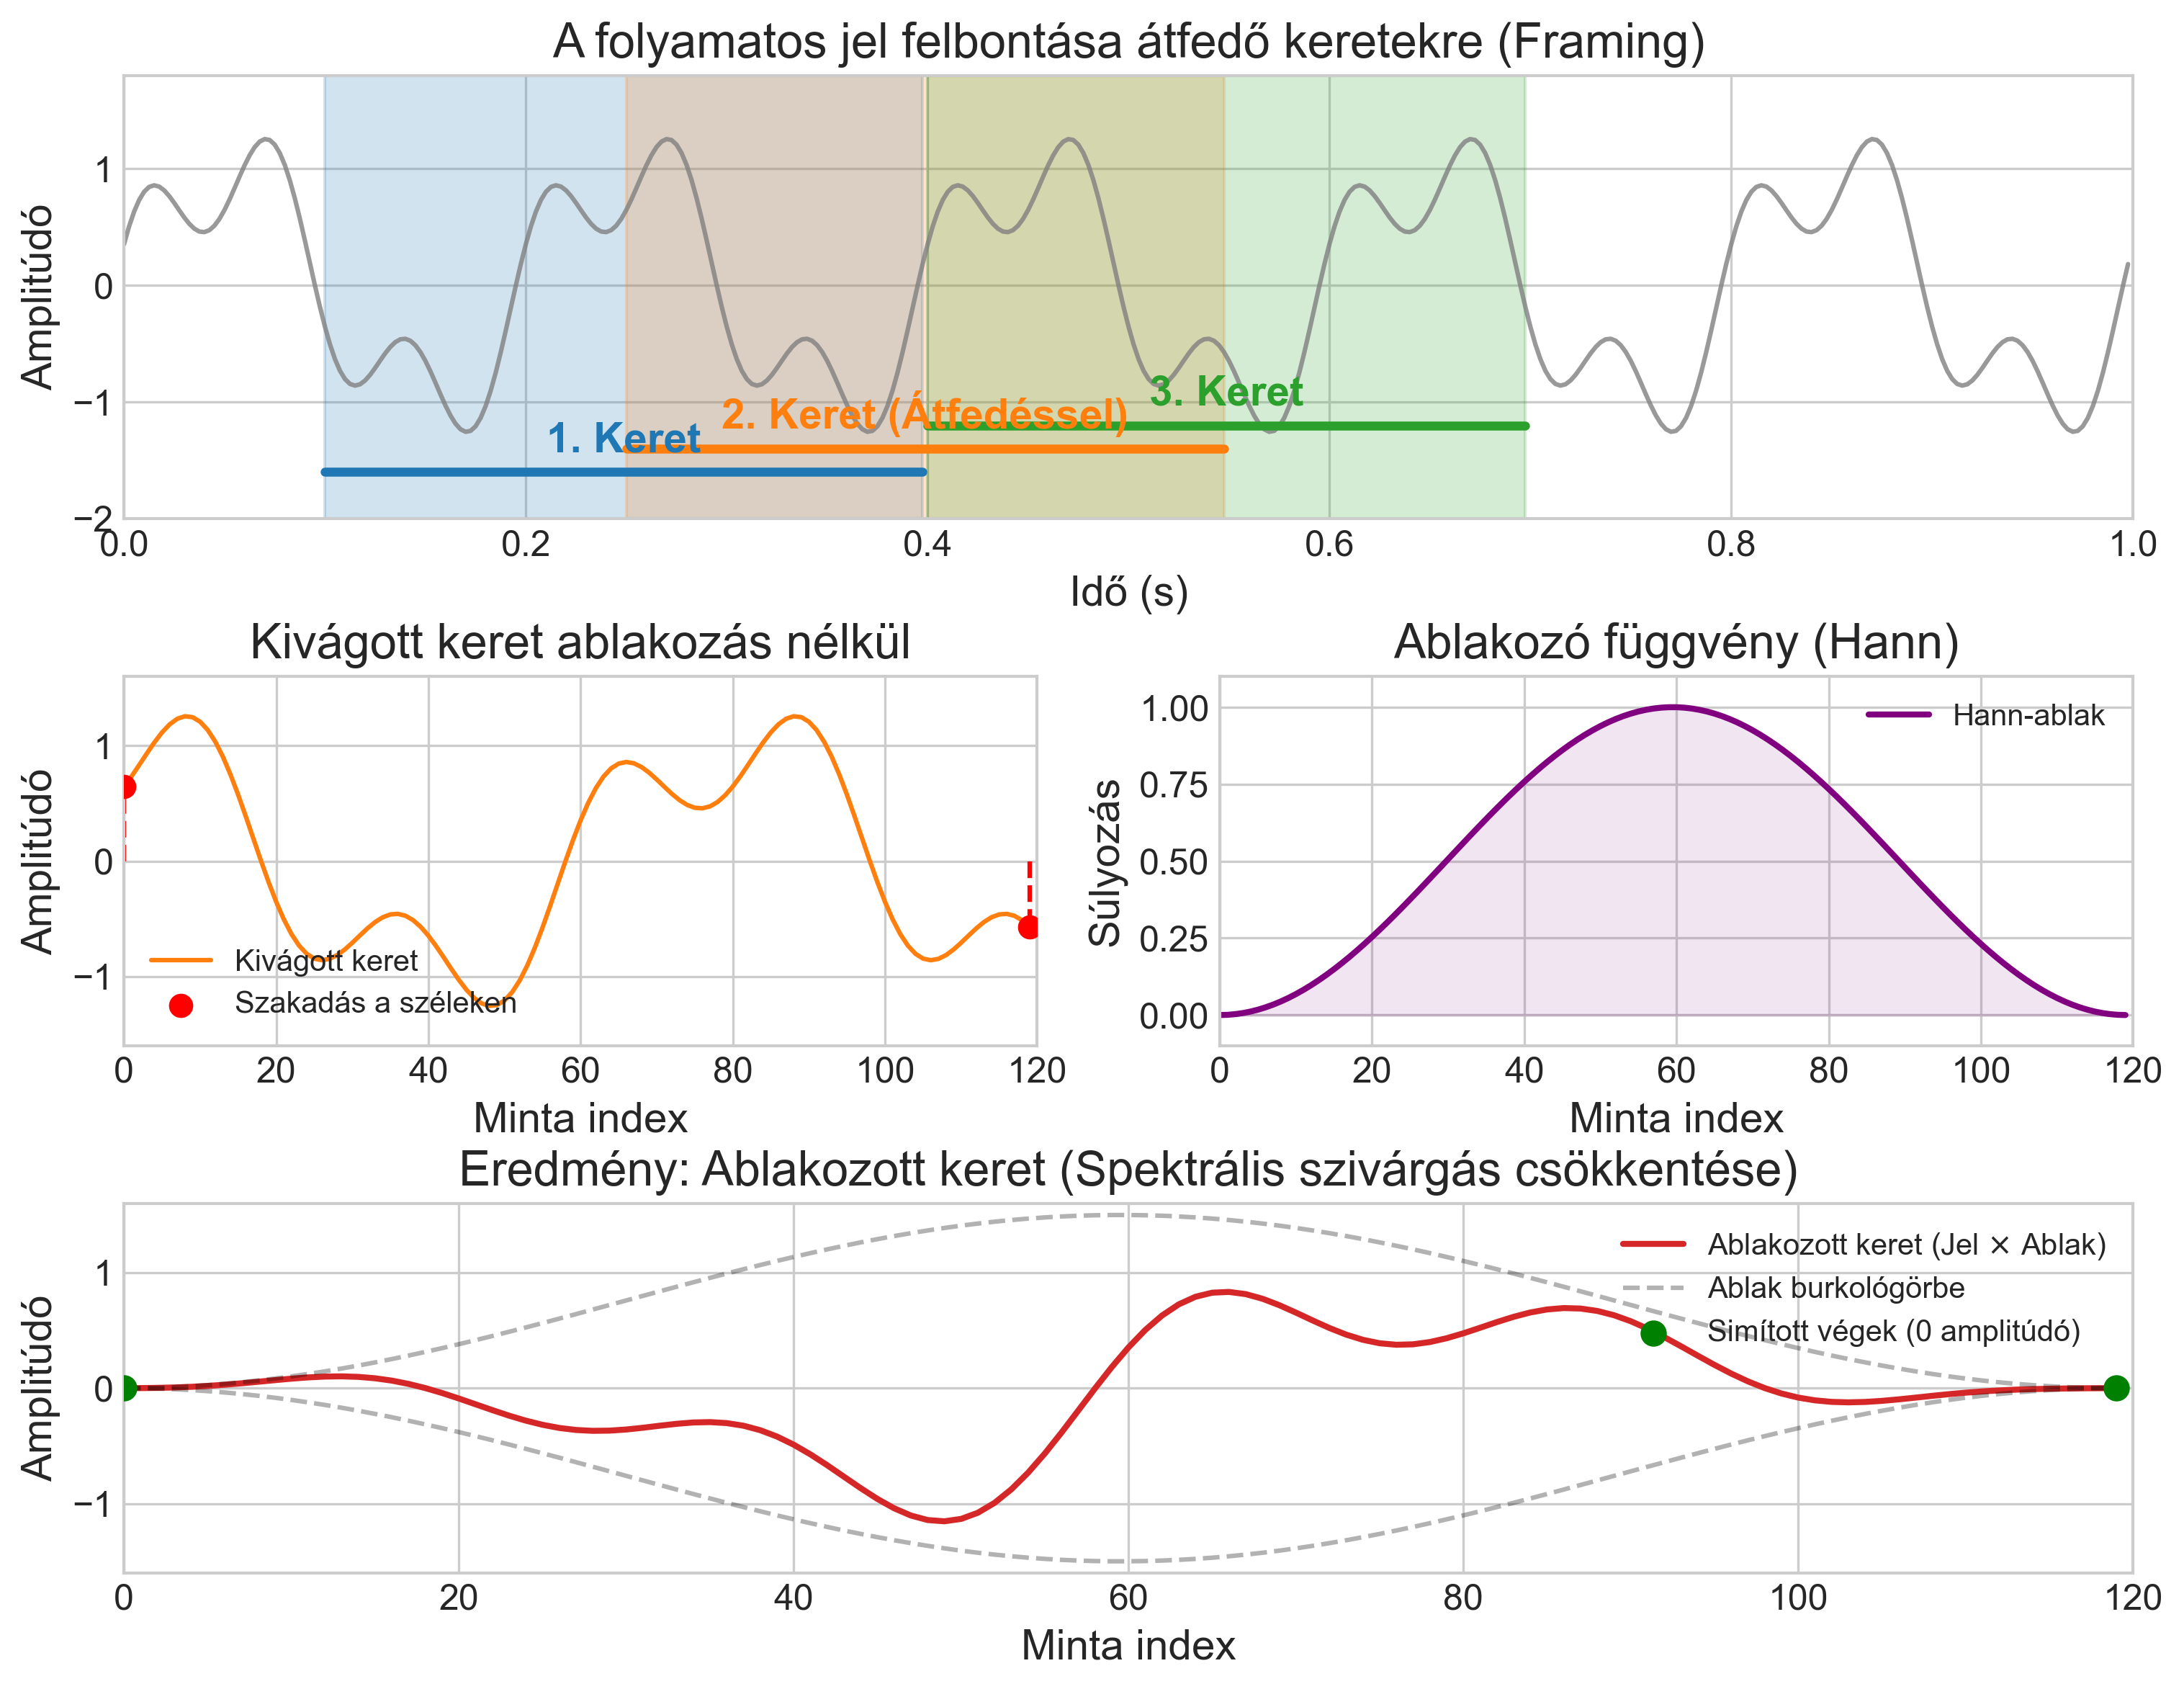
\includegraphics[width=0.82\textwidth]{fig_framing_windowing.png}
    \caption{A keretezés és ablakozás folyamata: a hangjelet rövid, átfedő ablakokra bontjuk, majd az egyes keretek széleit simítjuk.}
    \label{fig:framing_windowing}
\end{figure}

\section{Spektrogramok és tanulható bemenetek}
\label{sec:spektrogramok}

A nyers hullámforma közvetlenül is tartalmaz minden információt, de egy kis méretű saját modell számára nehezen tanulható bemenet. Ezért a hangot célszerű idő-frekvencia reprezentációvá alakítani. A rövid idejű Fourier-transzformáció (STFT) minden keretet frekvenciakomponensekre bont, az eredmény pedig egy spektrogram: egy képszerű mátrix, ahol az egyik tengely az időt, a másik a frekvenciát, a színintenzitás pedig az energiát jelöli.

\begin{figure}[H]
    \centering
    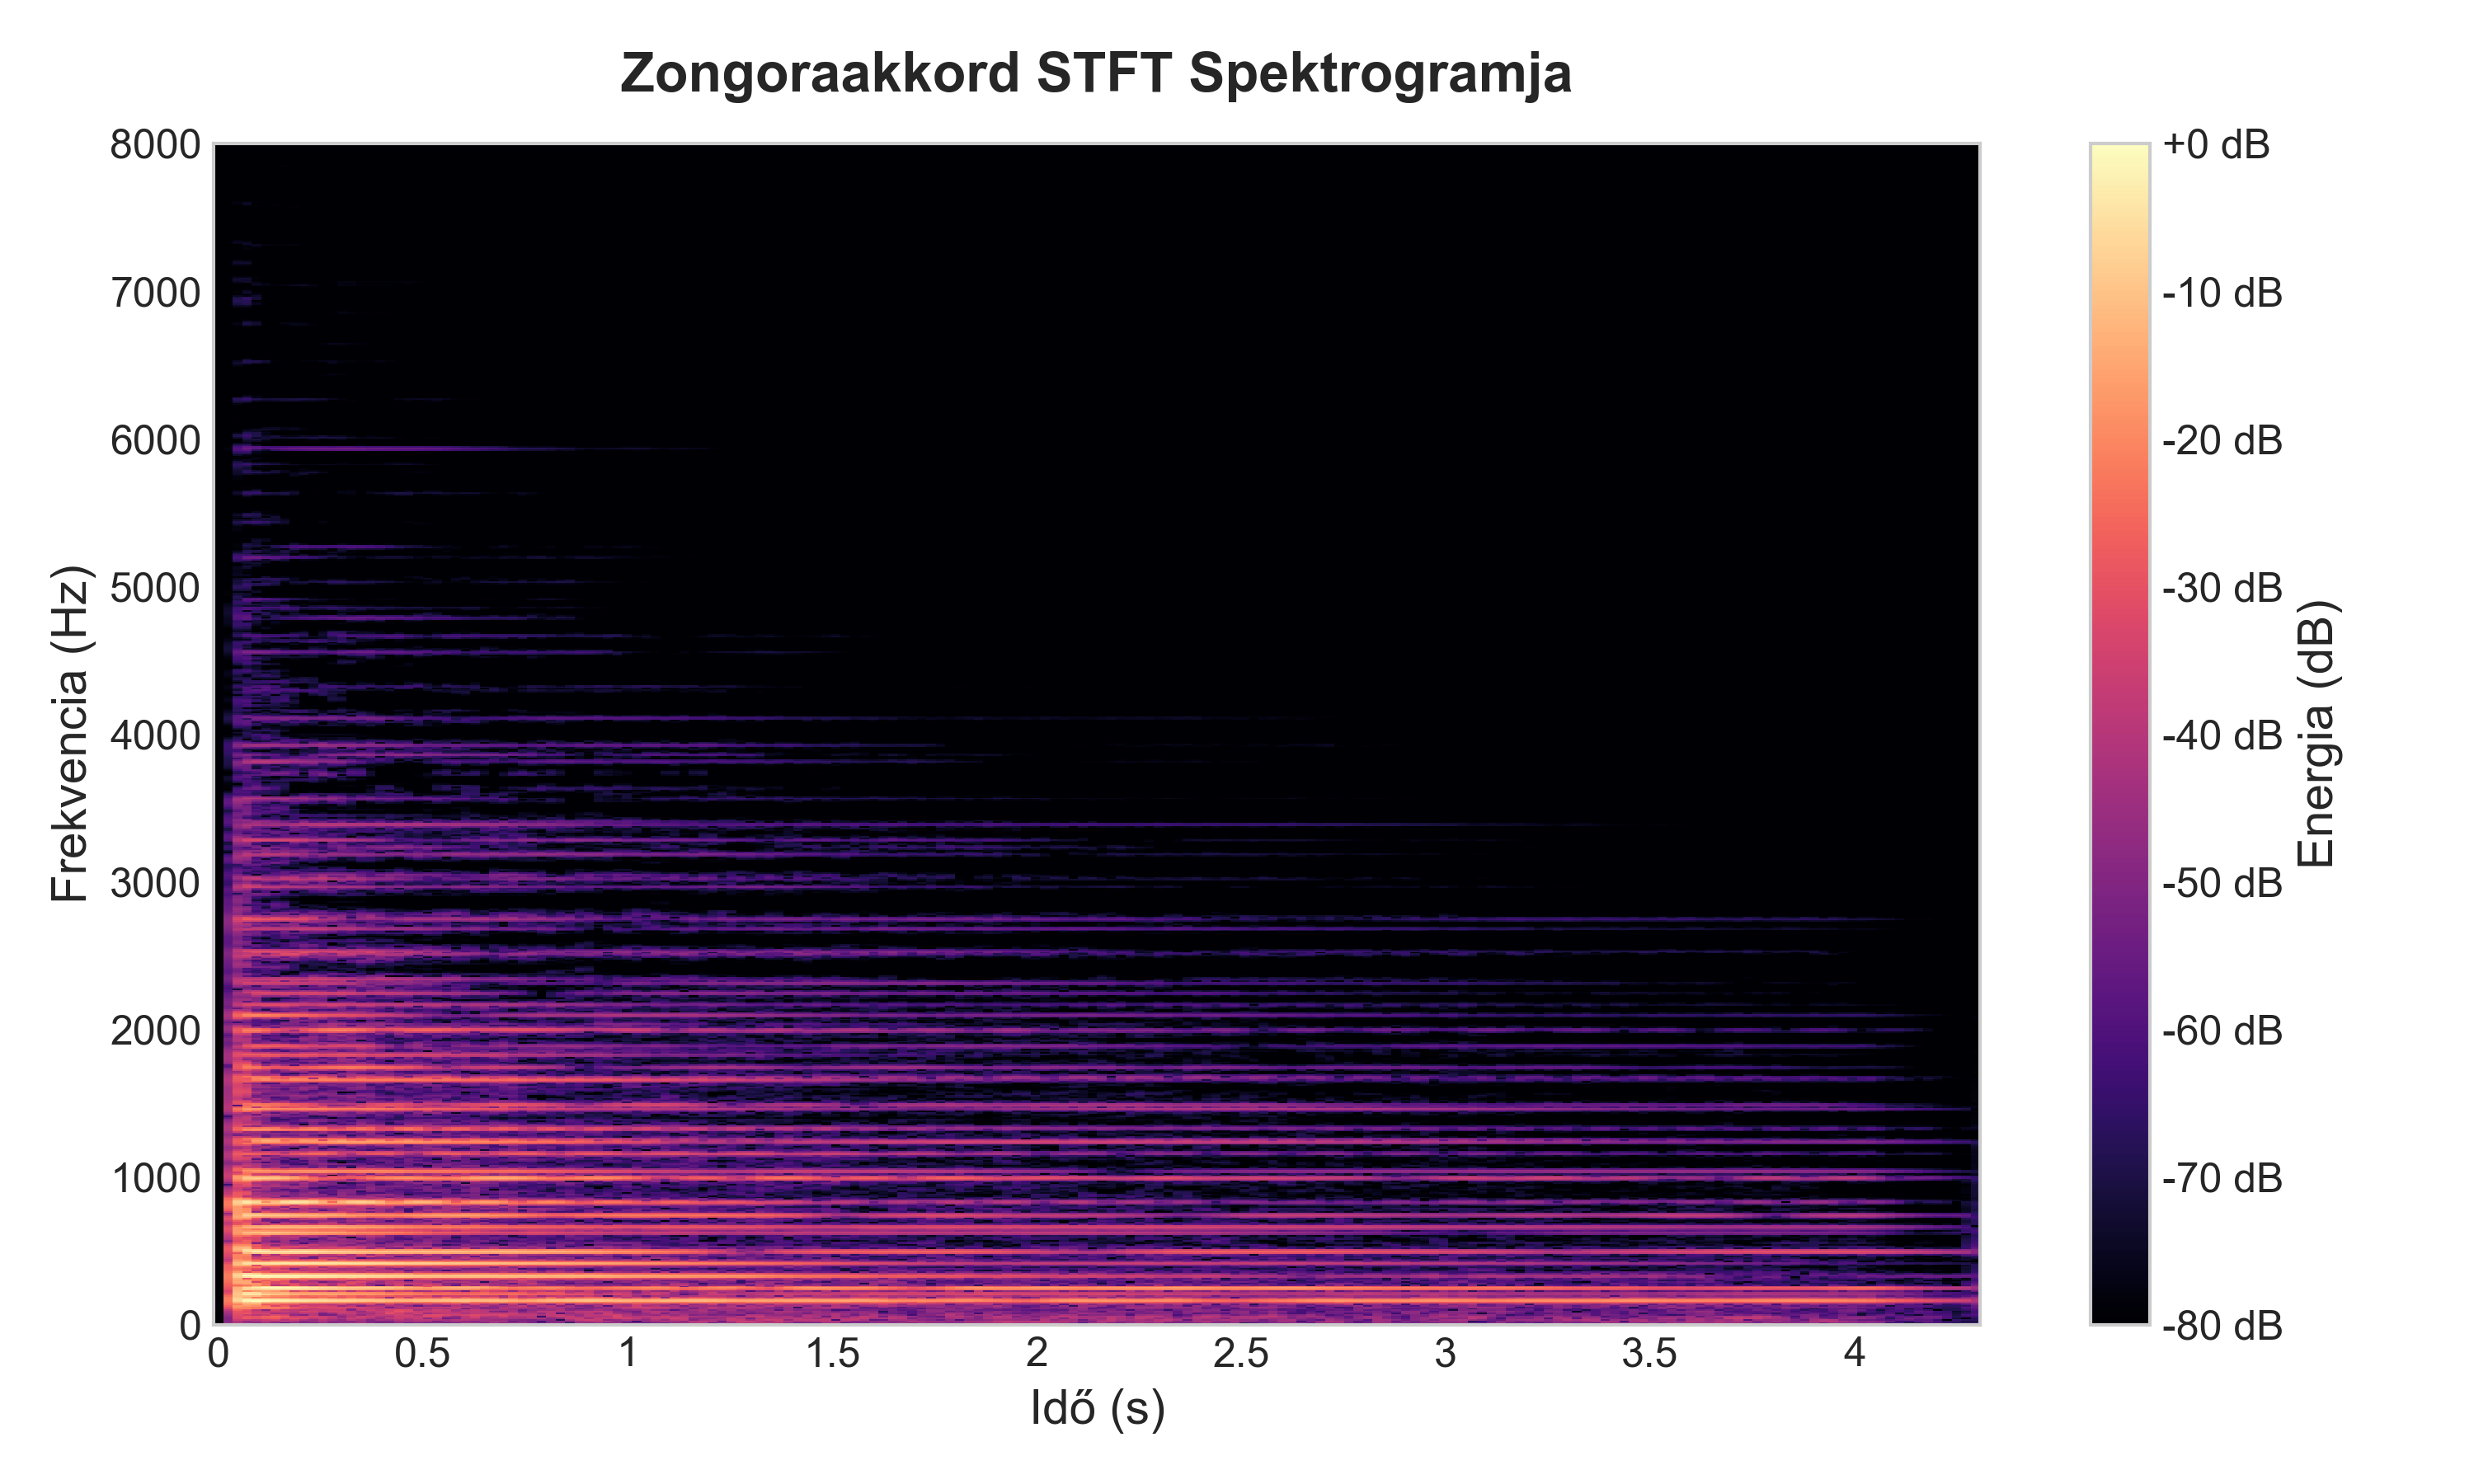
\includegraphics[width=0.78\textwidth]{fig_spectrogram_example.png}
    \caption{Egy rövid gitárhang hullámformája és STFT-spektrogramja. A spektrogramon az idő és frekvencia mentén láthatóvá válik, hol található a hang energiája.}
    \label{fig:spectrogram_example}
\end{figure}

A lineáris frekvenciaskála mellett gyakran használunk perceptuális skálákat is. Az emberi hallás az alacsony frekvenciák közötti különbségekre érzékenyebb, míg magas frekvenciákon kevésbé finom a megkülönböztetés. Ezt követi a Mel-skála: a mély tartományt részletesebben, a magas tartományt tömörebben ábrázolja. Ha az STFT után Mel-szűrőbankot és logaritmikus decibel skálázást alkalmazunk, log-Mel spektrogramot kapunk. A log-Mel bemenet zenei audiofeladatokban is gyakori, mert a CNN a spektrális és időbeli mintázatokat képszerű reprezentáción tanulhatja meg \cite{pons2018end}.

\begin{figure}[H]
    \centering
    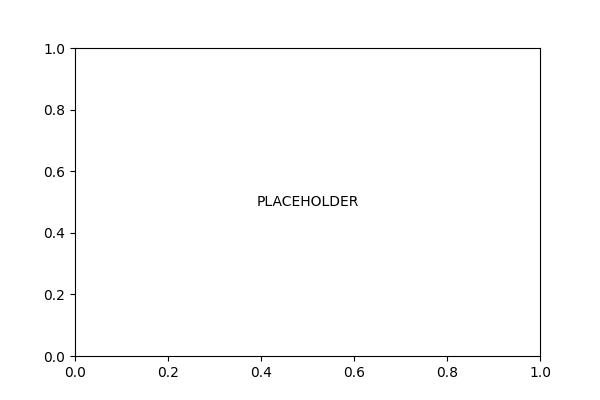
\includegraphics[width=0.82\textwidth]{fig_mel_vs_linear.png}
    \caption{Elméleti szemléltetés ugyanazon gitárhang lineáris STFT- és log-Mel spektrogramjával. A Mel-skála az emberi hallás frekvenciaérzékeléséhez igazítja a reprezentációt, ezért a mélyebb tartományt részletesebben kezeli.}
    \label{fig:mel_vs_linear}
\end{figure}

A dolgozatban három jellemzőkinyerési irányt használok összehasonlítási alapként. Az \textbf{STFT} közvetlen, lineáris frekvenciatengelyű spektrogramot ad, ezért alapvető frekvencia-idő baseline. Az \textbf{MFCC} klasszikus, tömörített audiojellemző, amely a Mel-spektrum diszkrét koszinusz transzformációjával keletkezik, és főleg hagyományos gépi tanulási feladatokban terjedt el. A \textbf{log-Mel spektrogram} a kettő között helyezkedik el: képszerű struktúrát őriz meg, de a frekvenciatengelyt az emberi halláshoz igazítja.

\begin{table}[H]
\centering
\caption{A három vizsgált bemeneti reprezentáció elméleti szerepe}
\label{tab:mfcc_vs_mel}
\begin{tabular}{p{2.6cm}p{4.0cm}p{6.4cm}}
\toprule
\textbf{Reprezentáció} & \textbf{Jelleg} & \textbf{Miért került be a dolgozatba?} \\
\midrule
STFT & Lineáris spektrogram & Megmutatja, hogyan teljesít a közvetlen frekvencia-idő ábrázolás. \\
MFCC & Tömörített kepsztrális jellemző & Klasszikus audio baseline, kisebb dimenzióval és erősebb előfeldolgozással. \\
Log-Mel & Perceptuális spektrogram & CNN-hez jól illeszkedő, képszerű és hallásközeli reprezentáció. \\
\bottomrule
\end{tabular}
\end{table}

\section{Neurális osztályozás spektrogramokon}
\label{sec:neuralis_osztalyozas}

A hangszerfelismerés felügyelt osztályozási feladat: minden tanítómintához tartozik egy bemenet és egy címke. A modell feladata, hogy a bemenet alapján hét kategória közül válasszon. Többosztályos neurális hálózatnál a kimeneti réteg tipikusan softmax aktivációt használ, amely minden osztályhoz egy valószínűségszerű értéket rendel. A prediktált osztály az lesz, amelynek a kimeneti értéke a legnagyobb.

A tanítás során a hálózat a hibás predikciók alapján módosítja a súlyait. A validációs halmaz szerepe az, hogy mérje: a modell nemcsak a tanítóadatokat jegyezte-e meg, hanem új mintákon is képes-e általánosítani. A túlilleszkedés (overfitting) akkor jelenik meg, amikor a modell a tanítóhalmazon jól teljesít, de a validációs vagy teszthalmazon gyengébben. Ennek mérséklésére használhatók például dropout rétegek, adataugmentáció, címkesimítás, valamint korai leállítás. Spektrogram-bemeneteknél az idő- és frekvenciamaszkok használata a SpecAugment módszerrel vált ismertté \cite{park2019specaugment}; a saját rendszerben ennek egyszerűsített gondolata jelenik meg tanítás közbeni maszkolásként.

Spektrogramok esetében a 2D konvolúciós neurális hálózat természetes választás, mert a bemenet képszerű: az egyik tengely az időt, a másik a frekvenciát jelöli. A konvolúciós szűrők lokális idő-frekvencia mintázatokat tanulnak, például hirtelen tranzienseket, kitartott harmonikus sávokat vagy zajos spektrális tartományokat.

Nem állítom, hogy a 2D CNN minden alternatívánál általánosan jobb. Egy SVM vagy más klasszikus modell használható lehet kézzel aggregált jellemzővektorokon, egy MLP viszont a spektrogram kilapításával elveszítené a lokális szerkezetet. Az 1D CNN inkább nyers hullámformán vagy időbeli jellemzősorozaton természetes, a CRNN pedig erősebb időbeli modellezést adhat, de összetettebb és több magyarázati terhet jelent. A saját rendszerben a 2D CNN ezért arányos kompromisszum: illeszkedik a log-Mel bemenethez, kezelhető méretű, és valós időben is futtatható.

\section{Hangszercsaládok akusztikai szemléltetése}
\label{subsec:hangszercsaladok}

A rendszer nem egyedi hangszereket, hanem hangszercsaládokat különít el. Ez a döntés akusztikailag is indokolható: az egy családba tartozó hangszerek azonos vagy hasonló hangkeltési elvük miatt rokon időbeli és spektrális mintázatokat mutathatnak. A kis adathalmaz és a valós idejű cél miatt ez a csoportosítás védhetőbb, mint sok különálló hangszerosztály kezelése.

\begin{table}[H]
\centering
\caption{A rendszerben használt hangszercsaládok és jellegzetes hullámformáik}
\label{tab:instrument_families}
\begingroup
\footnotesize
\setlength{\tabcolsep}{3pt}
\renewcommand{\arraystretch}{1.02}
\newcommand{\waveformcell}[1]{\includegraphics[width=\linewidth,height=0.72cm,keepaspectratio]{#1}}
\begin{tabular}{@{}>{\raggedright\arraybackslash}p{1.55cm}
                >{\raggedright\arraybackslash}p{2.15cm}
                >{\raggedright\arraybackslash}p{2.35cm}
                >{\raggedright\arraybackslash}p{4.35cm}
                >{\centering\arraybackslash}p{2.20cm}@{}}
\toprule
\textbf{Osztály} & \textbf{Példák} & \textbf{Hangkeltés} & \textbf{Jelleg} & \textbf{Hullámforma} \\
\midrule
Gitár & Akusztikus, elektromos gitár & Húr pengetése & Gyors attack, majd lecsengő rezgés. & \waveformcell{fig_table_guitar.png} \\
\midrule
Zongora & Zongora, e-piano & Kalapács által leütött húr & Impulzusszerű kezdet, hosszabb lecsengés. & \waveformcell{fig_table_piano.png} \\
\midrule
Vokál & Énekhang, torokének & Hangszálak rezgése & Kváziperiodikus jel, formánsokkal. & \waveformcell{fig_table_vocal.png} \\
\midrule
Vonós & Hegedű, brácsa, cselló, nagybőgő & Vonó és húr súrlódása & Kitartott, folytonos gerjesztés. & \waveformcell{fig_table_string.png} \\
\midrule
Nádfúvós & Klarinét, szaxofon, oboa, fagott & Nád rezgése & Kitartott, periodikus, rezonáns jel. & \waveformcell{fig_table_reed.png} \\
\midrule
Rézfúvós & Trombita, harsona, kürt, tuba & Ajkak rezgése fúvókán & Erős harmonikus szerkezet, nagy energia. & \waveformcell{fig_table_brass.png} \\
\midrule
Zaj/Csend & Környezeti zajok & Véletlenszerű rezgések & Aperiodikus, rendszertelen jel. & \waveformcell{fig_table_noise.png} \\
\bottomrule
\end{tabular}
\endgroup
\end{table}

A táblázatban hosszabb hullámforma-részletek szerepelnek, mert ezeken jól látszik a hang felfutása és lecsengése. Emellett kontrollált, közeli referenciahangokból külön nagyított példákat is készítettem. A legtöbb hangszer esetében A4 hangot használtam, a nagybőgő és a tuba esetében A3-at, mert ezeknél ez természetesebb regiszter. Ezek az ábrák nem tanítóadatok, hanem szemléltető példák: a periódus belső alakjára és a családon belüli hasonlóságokra nagyítanak rá.

\begin{figure}[H]
\centering
\begin{minipage}{0.48\textwidth}
    \centering
    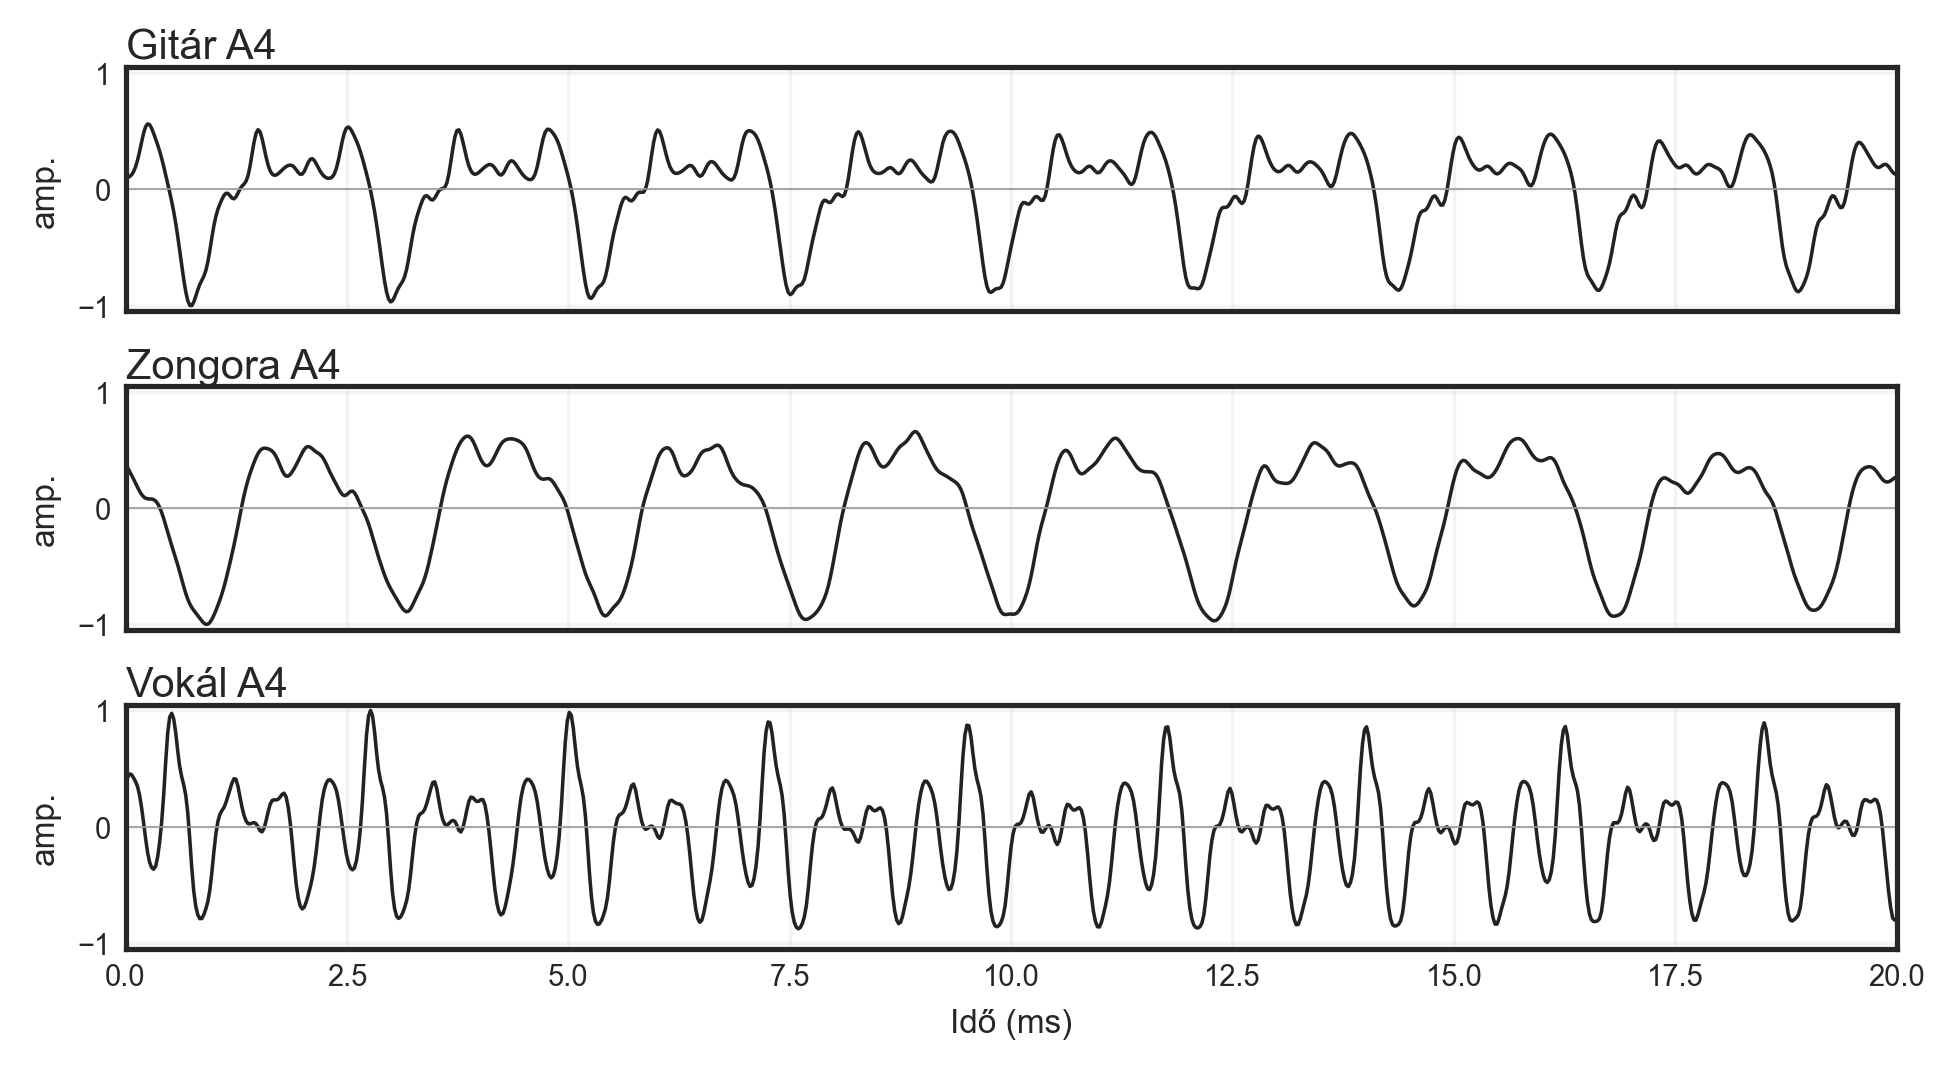
\includegraphics[width=\linewidth]{fig_asd_waveforms_solo.png}
    \footnotesize (a) Gitár, zongora és vokál
\end{minipage}\hfill
\begin{minipage}{0.48\textwidth}
    \centering
    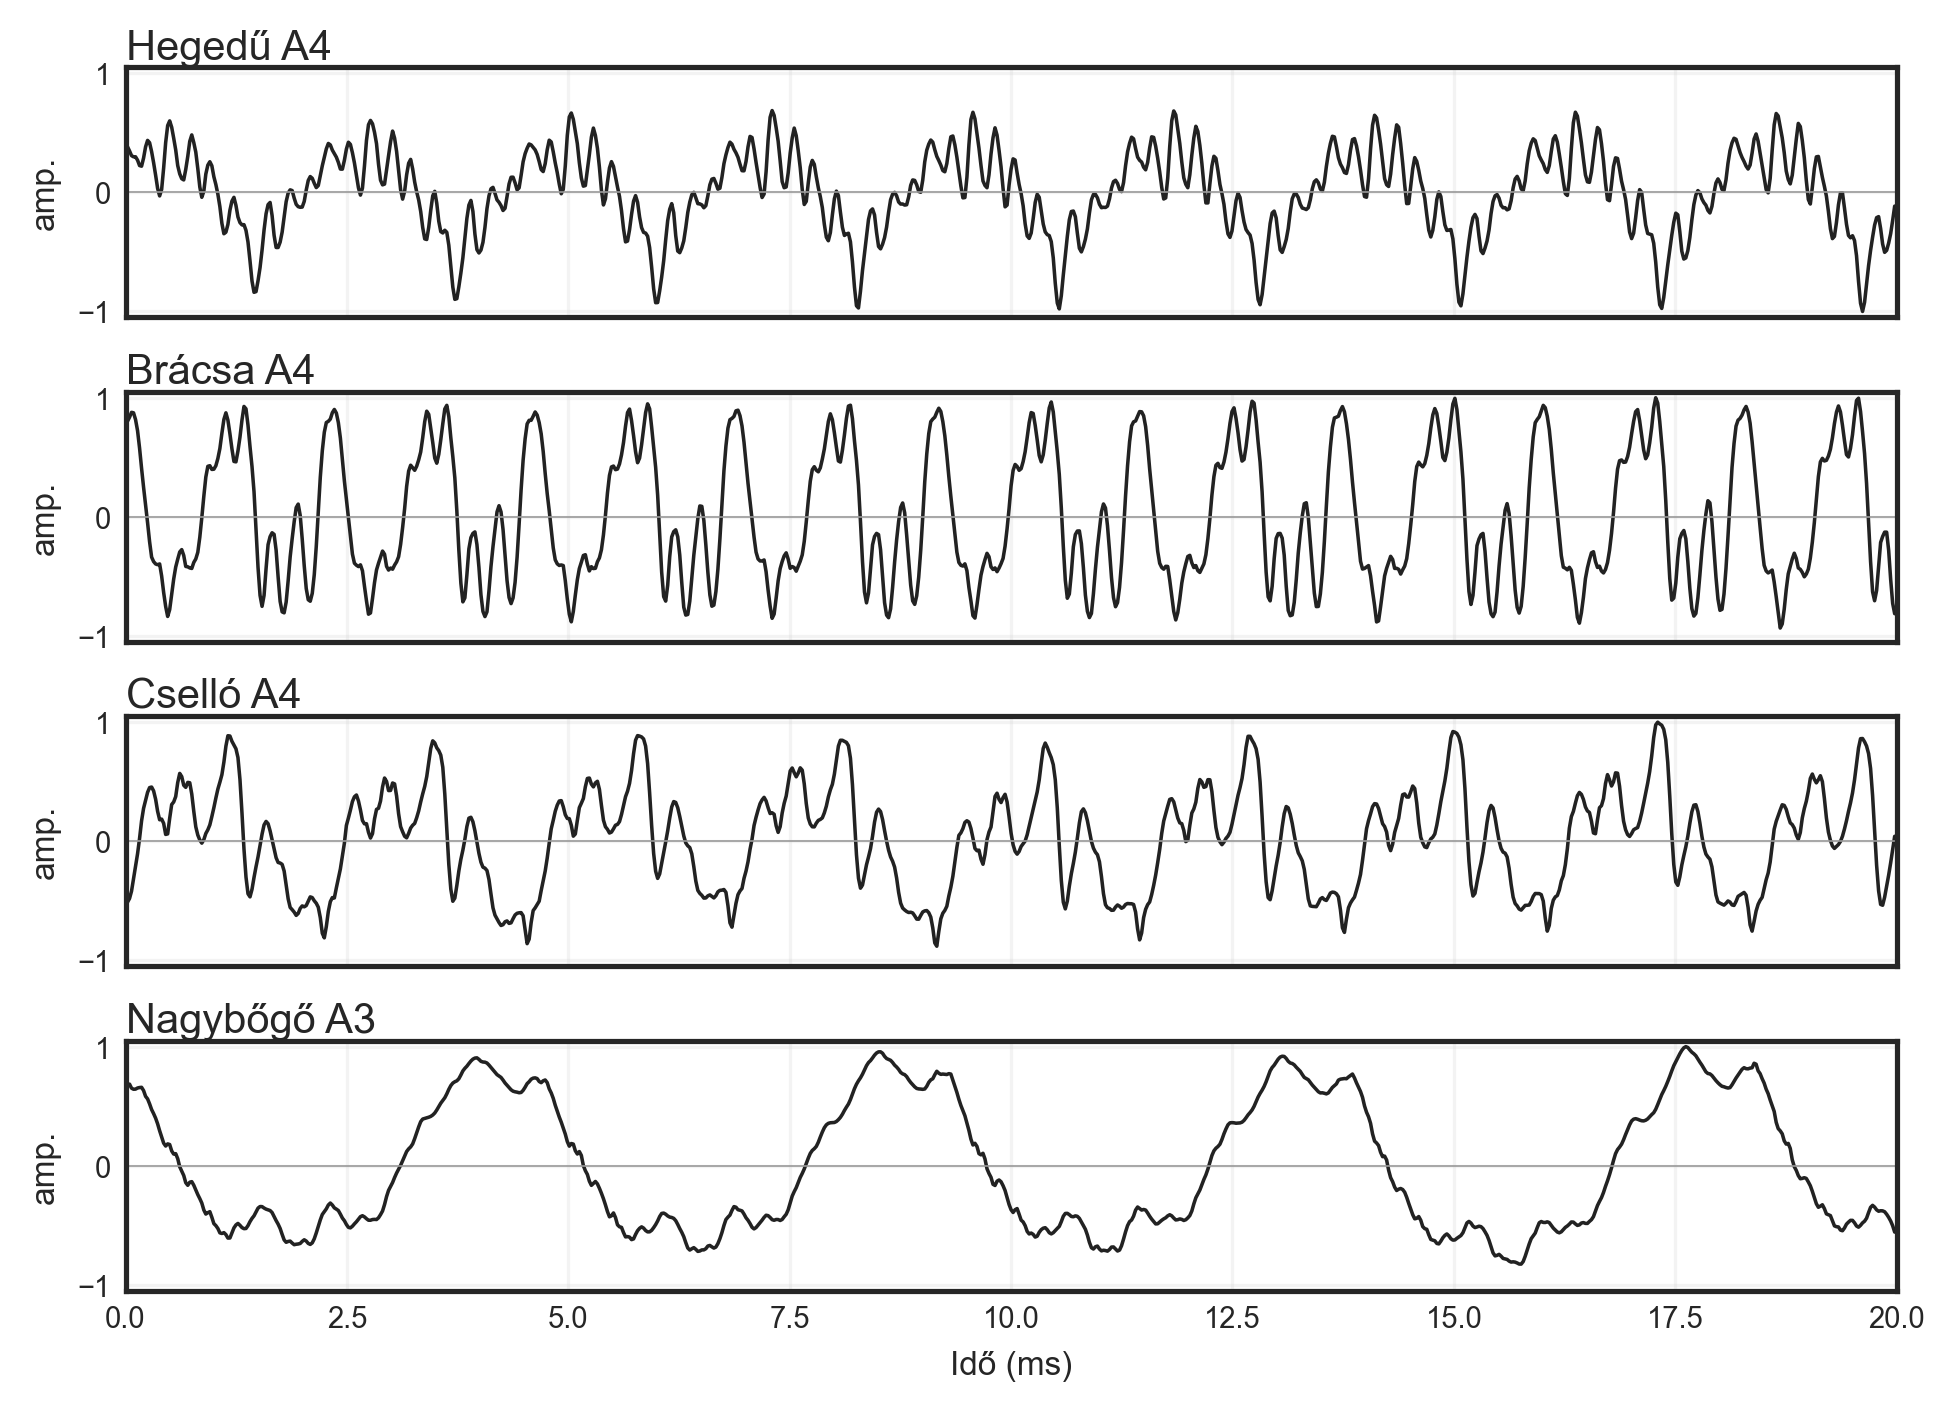
\includegraphics[width=\linewidth]{fig_asd_waveforms_string.png}
    \footnotesize (b) Vonós hangszerek
\end{minipage}

\vspace{0.4cm}

\begin{minipage}{0.48\textwidth}
    \centering
    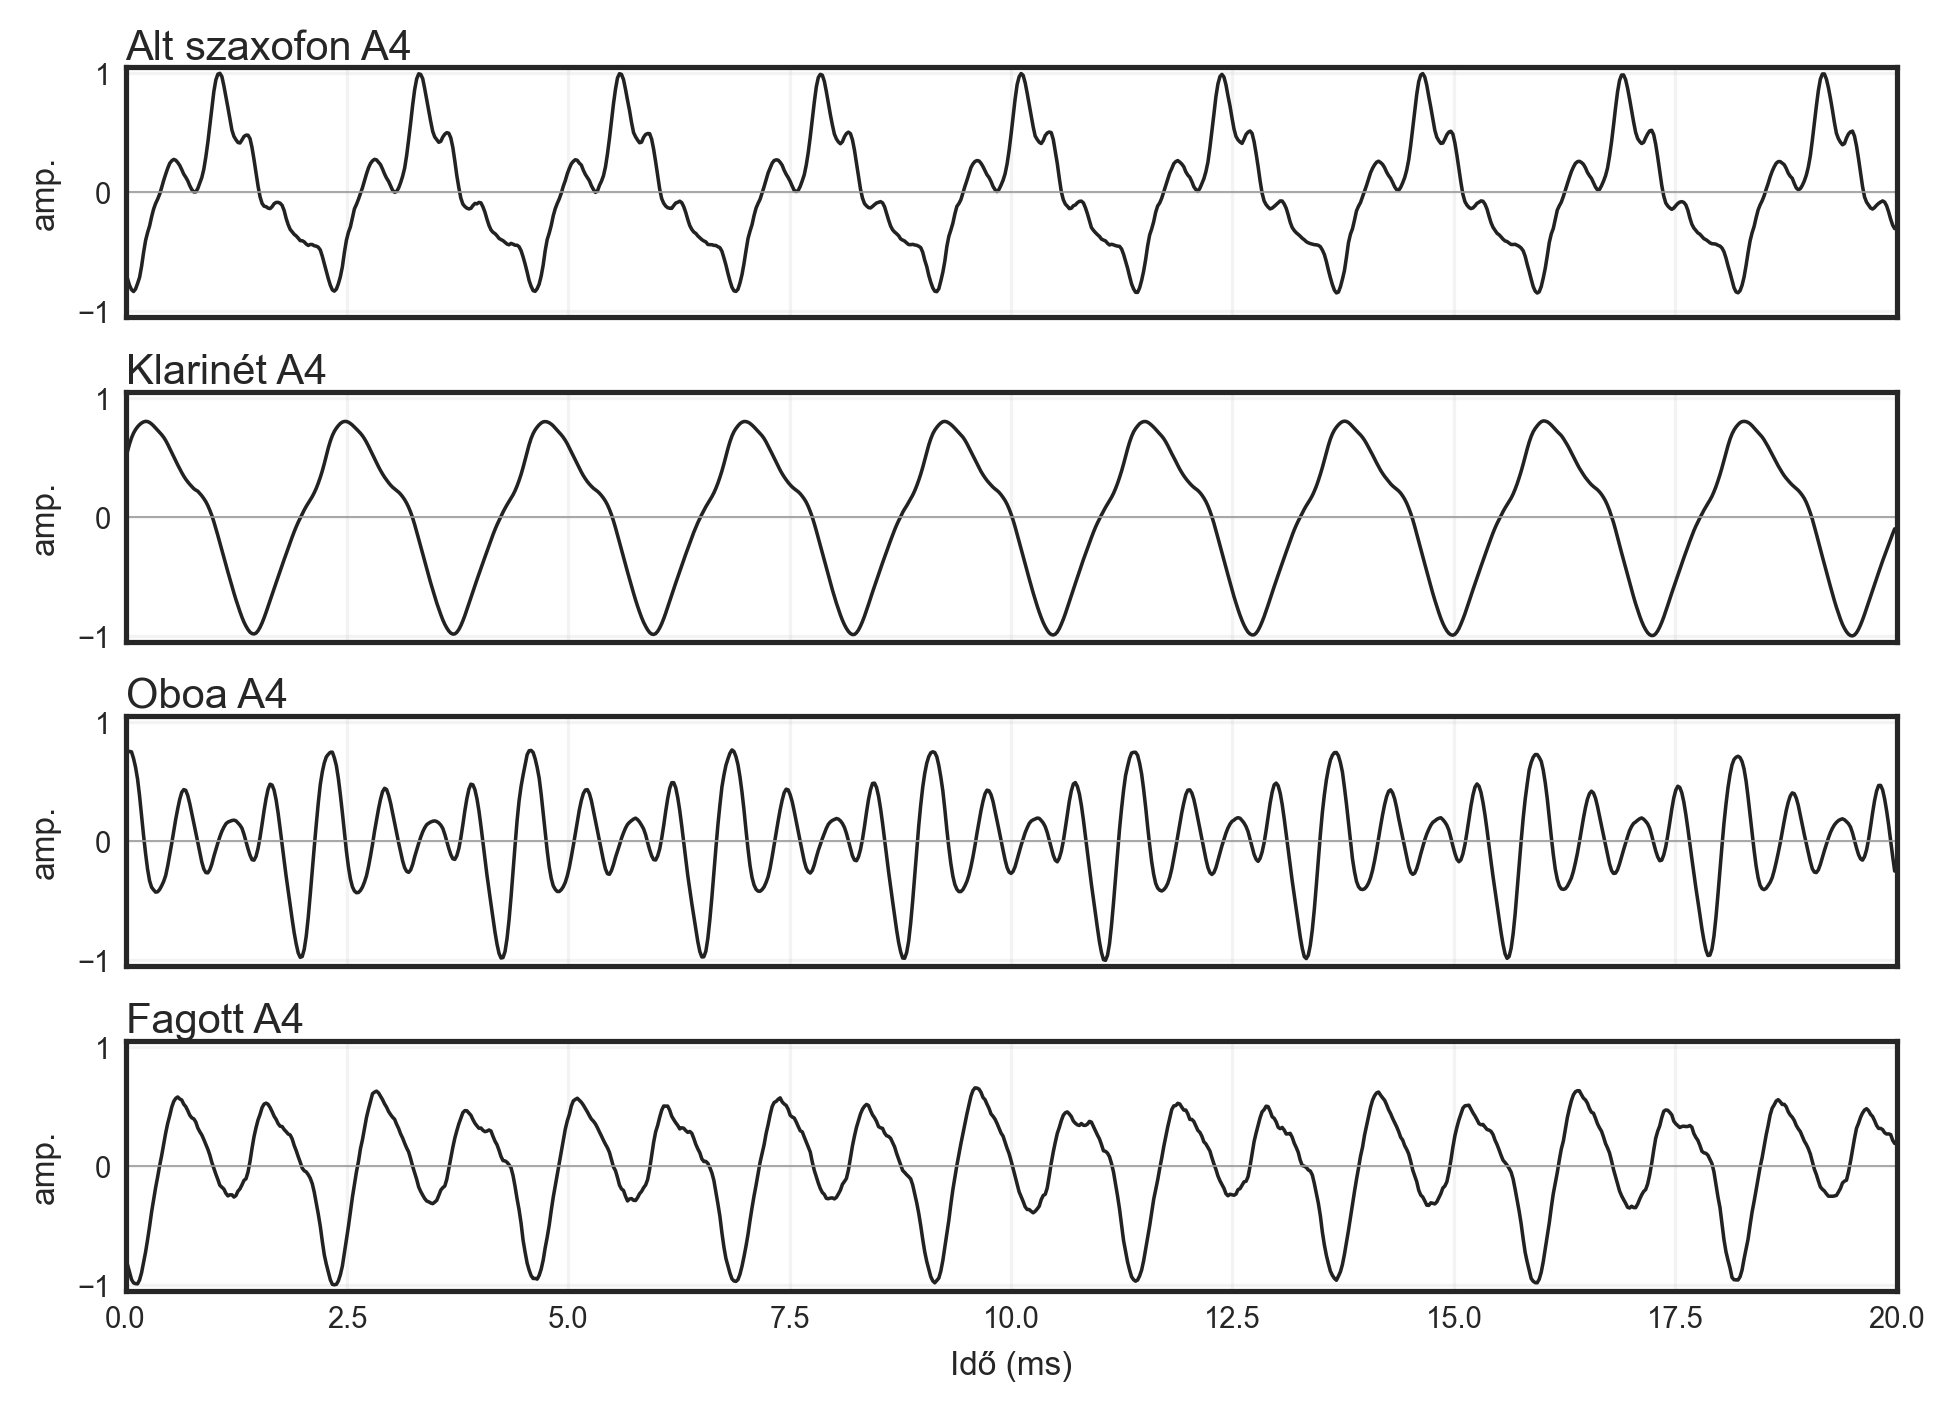
\includegraphics[width=\linewidth]{fig_asd_waveforms_reed.png}
    \footnotesize (c) Nádfúvós hangszerek
\end{minipage}\hfill
\begin{minipage}{0.48\textwidth}
    \centering
    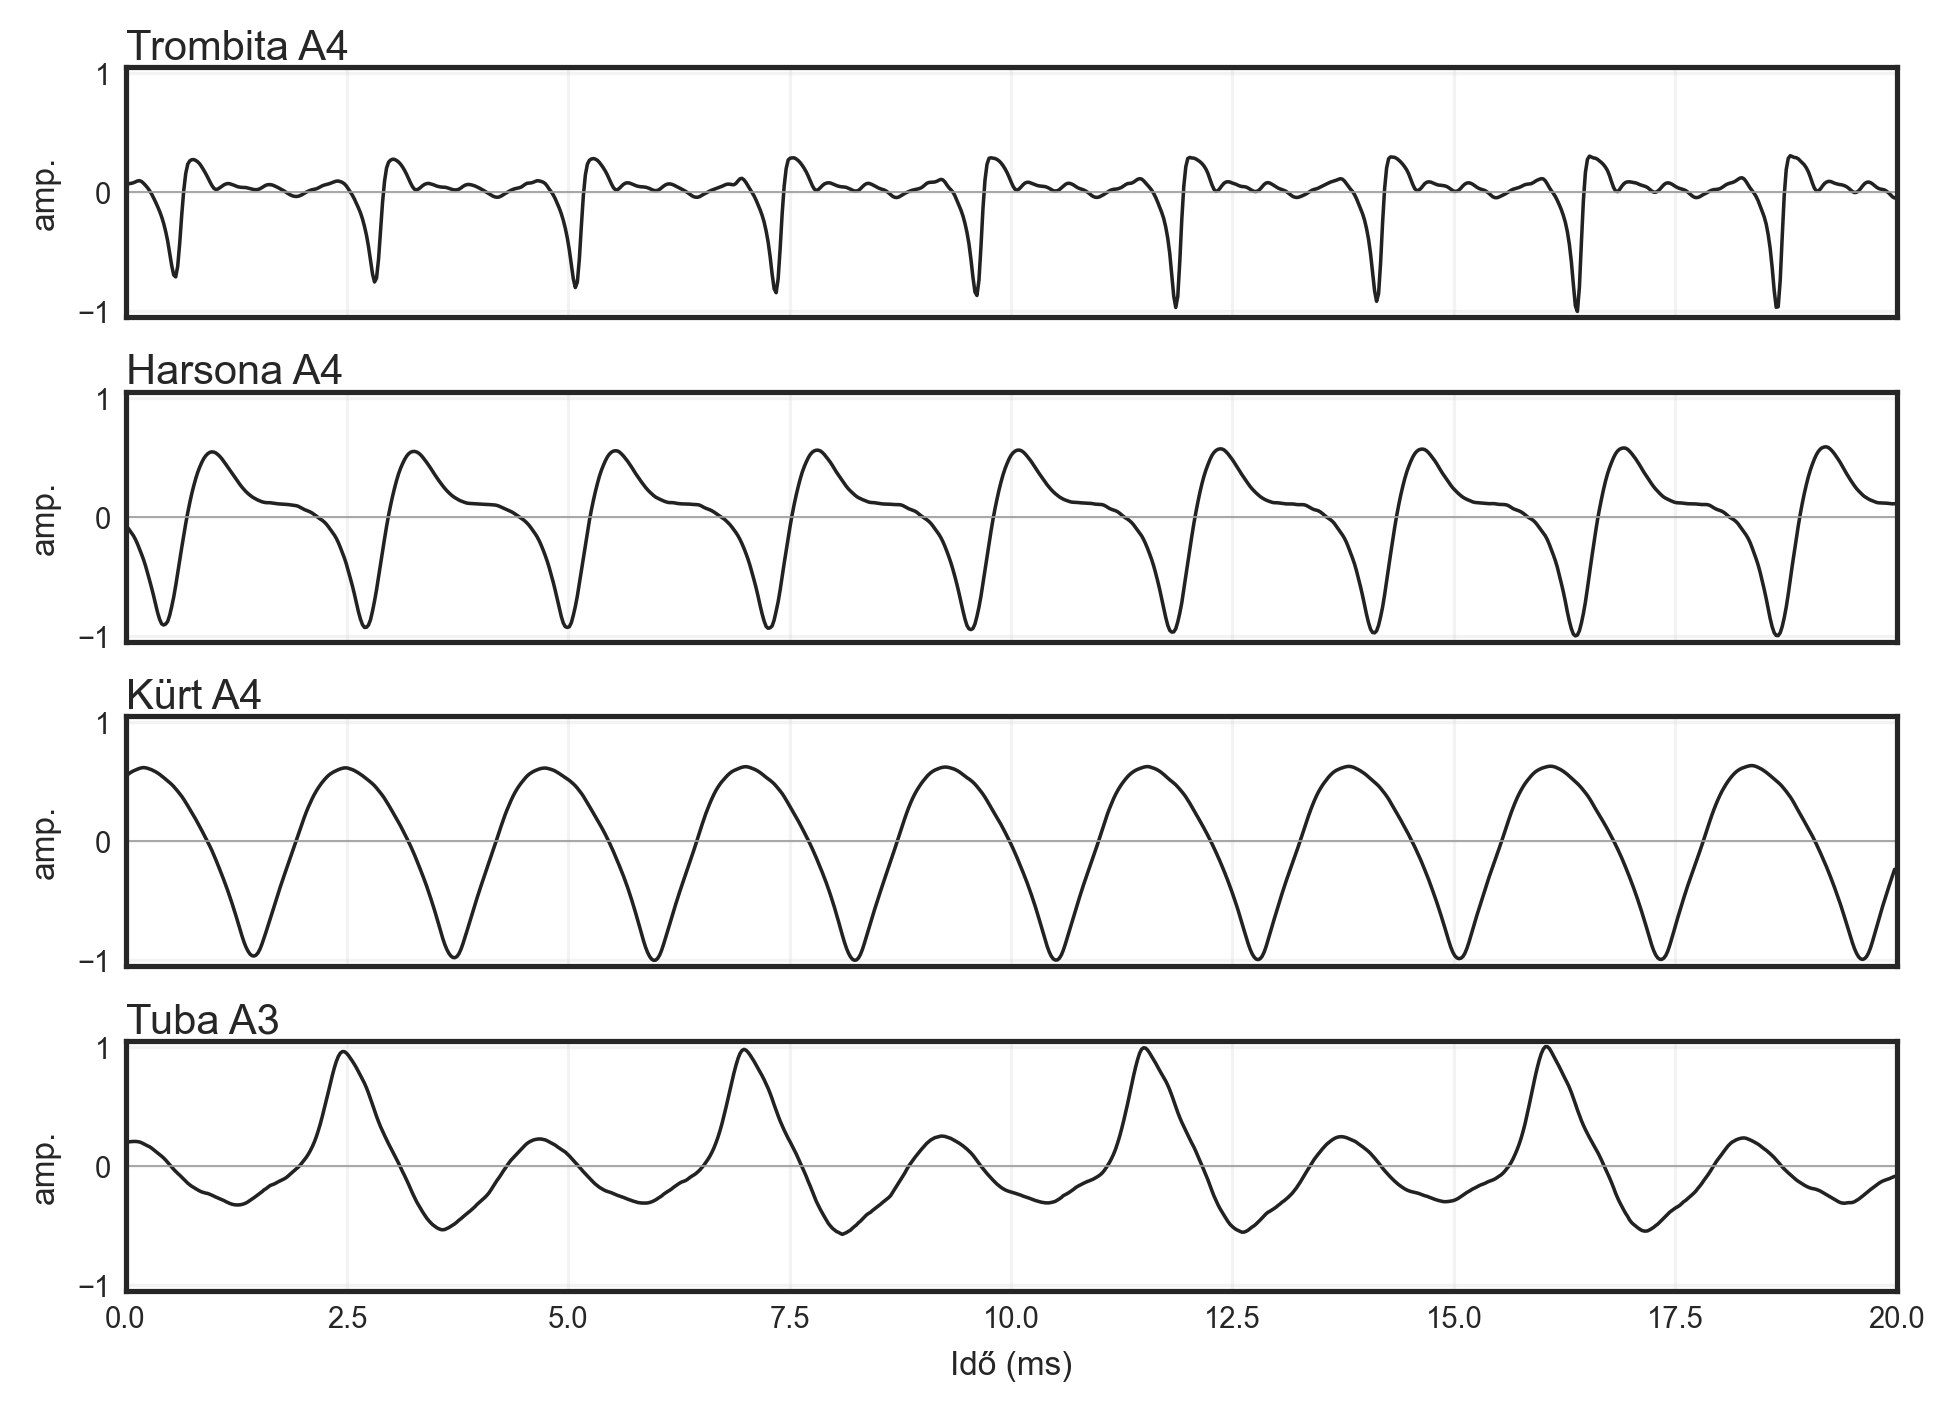
\includegraphics[width=\linewidth]{fig_asd_waveforms_brass.png}
    \footnotesize (d) Rézfúvós hangszerek
\end{minipage}
\caption{Kontrollált A4/A3 referenciahangok 20 ms-os nagyított hullámforma-részletei. A cél nem a hangerő, hanem a periodicitás és a jelalak családonkénti szemléltetése.}
\label{fig:asd_waveforms_summary}
\end{figure}

\section{Validációs kockázatok: leakage, domain shift, domain adaptation}
\label{sec:adatszivargas_elmelet}

Gépi tanulási rendszereknél a kiértékelés egyik legfontosabb kockázata az adatszivárgás, vagyis amikor a modell a tanítás során olyan információhoz jut, amely a valós használat során nem lenne elérhető. Audio esetén ez különösen könnyen előfordulhat, mert egy hosszabb felvétel egymáshoz közeli szeletei nagyon hasonlóak lehetnek. Ha ezek egyszerre kerülnek train és test halmazba, a modell túl optimista eredményt adhat.

A dolgozat szempontjából három leakage-típust érdemes kiemelni. A \textbf{train-test kontamináció} akkor jelenik meg, ha nagyon hasonló vagy azonos minták kerülnek különböző splitbe. Az \textbf{előfeldolgozási leakage} akkor fordul elő, ha például normalizálási paramétereket a teljes adathalmazból számolunk, majd azokat a tesztadatokra is alkalmazzuk. Az \textbf{augmentációs leakage} pedig akkor veszélyes, ha egy eredeti minta az egyik, annak torzított változata pedig egy másik halmazba kerül.

A valós idejű mikrofonos felismerésnél emellett megjelenik a \textbf{domain shift} is. Ez azt jelenti, hogy a tanítási környezet és a célkörnyezet eloszlása eltér: a tiszta internetes vagy stúdiószerű hangok másképp viselkednek, mint a telefonról visszajátszott és laptopmikrofonnal rögzített minták. A \textbf{domain adaptation} ennek kezelésére szolgál: a célkörnyezetből származó mikrofonos train minták bevonásával a modell jobban alkalmazkodhat ahhoz az akusztikai helyzethez, amelyben később működnie kell.

Ezek miatt a későbbi kísérletekben a train, validation és test halmazokat külön szerepben kezelem. A validáció a modellválasztásra szolgál, a test halmaz pedig csak a kiválasztott végső modellek utolsó ellenőrzésére. Így a mérési eredmények nem rekordpontosságként, hanem kontrollált, módszertanilag védhető összehasonlításként értelmezhetők.
